\documentclass{article}
\usepackage{amssymb,amsmath}
\usepackage{ifxetex,ifluatex}
\ifxetex
  \usepackage{fontspec,xltxtra,xunicode}
  \defaultfontfeatures{Mapping=tex-text,Scale=MatchLowercase}
\else
  \ifluatex
    \usepackage{fontspec}
    \defaultfontfeatures{Mapping=tex-text,Scale=MatchLowercase}
  \else
    \usepackage[utf8]{inputenc}
  \fi
\fi
\usepackage{ctable}
\usepackage{float} % provides the H option for float placement
\usepackage{graphicx}
% We will generate all images so they have a width \maxwidth. This means
% that they will get their normal width if they fit onto the page, but
% are scaled down if they would overflow the margins.
\makeatletter
\def\maxwidth{\ifdim\Gin@nat@width>\linewidth\linewidth
\else\Gin@nat@width\fi}
\makeatother
\let\Oldincludegraphics\includegraphics
\renewcommand{\includegraphics}[1]{\Oldincludegraphics[width=\maxwidth]{#1}}
\ifxetex
  \usepackage[setpagesize=false, % page size defined by xetex
              unicode=false, % unicode breaks when used with xetex
              xetex]{hyperref}
\else
  \usepackage[unicode=true]{hyperref}
\fi
\hypersetup{breaklinks=true, pdfborder={0 0 0}}
\setlength{\parindent}{0pt}
\setlength{\parskip}{6pt plus 2pt minus 1pt}
\setlength{\emergencystretch}{3em}  % prevent overfull lines
\setcounter{secnumdepth}{0}

\title{Descriptives}
\author{Rapport package team @ https://github.com/aL3xa/rapport}
\date{2011--04--26 20:25 CET}

\begin{document}
\maketitle

\subsection{Description}

This template will return descriptive statistics of numerical, or
frequency tables of categorical variables.

\subsubsection{\emph{gender} (``Gender'')}

The dataset has 709 observations with 673 valid values (missing: 36) in
\emph{gender} (``Gender''). This variable seems to be a factor.

\paragraph{Base statistics}

\ctable[pos = H, center, botcap]{llllll}
{% notes
}
{% rows
\FL
 & \textbf{gender} & \textbf{N} & \textbf{pct} & \textbf{cumul.count} & \textbf{cumul.pct}
\ML
1 & male & 410.00 & 60.92 & 410.00 & 60.92
\\\noalign{\medskip}
2 & female & 263.00 & 39.08 & 673.00 & 100.00
\\\noalign{\medskip}
Total &  & 673.00 & 100.00 & 673.00 & 100.00
\LL
}

\paragraph{Barplot}

\begin{figure}[htbp]
\centering
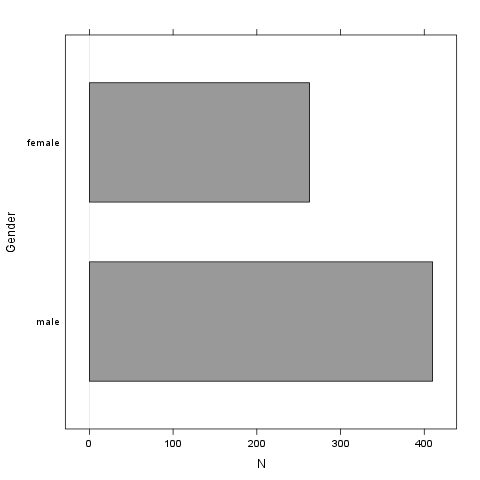
\includegraphics{3ed92ab3ffc6e875335e7e8c774c35a8.png}
\caption{}
\end{figure}

It seems that the highest value is 2 which is exactly 2 times higher
than the smallest value (1).

\subsubsection{\emph{age} (``Age'')}

The dataset has 709 observations with 677 valid values (missing: 32) in
\emph{age} (``Age''). This variable seems to be numeric.

\paragraph{Base statistics}

\ctable[pos = H, center, botcap]{llll}
{% notes
}
{% rows
\FL
\textbf{value} & \textbf{mean(age)} & \textbf{sd(age)} & \textbf{var(age)}
\ML
(all) & 24.57 & 6.85 & 46.91
\LL
}

\paragraph{Histogram}

\begin{figure}[htbp]
\centering
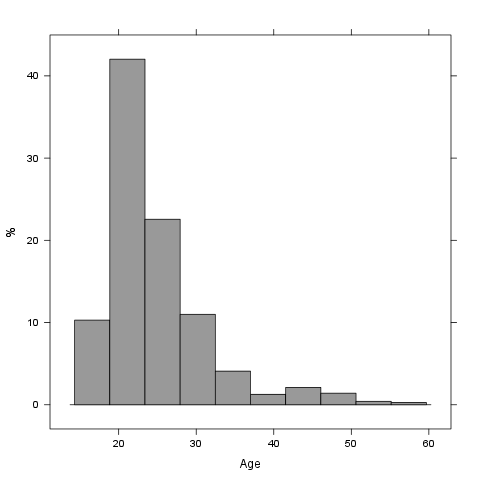
\includegraphics{ac5d789145bdef09b10219ef16429f53.png}
\caption{}
\end{figure}

It seems that the highest value is 58 which is exactly 3.625 times
higher than the smallest value (16).

The standard deviation is 6.8491 (variance: 46.911). The expected value
is around 24.573, somewhere between 24.057 and 25.089 (SE: 0.2632).

If we suppose that \emph{Age} is not near to a normal distribution
(test: , skewness: 1.9296, kurtosis: 7.4851), checking the median (23)
might be a better option instead of the mean. The interquartile range
(6) measures the statistics dispersion of the variable (similar to
standard deviation) based on median.

\subsection{Description}

This template will return descriptive statistics of numerical, or
frequency tables of categorical variables.

\subsubsection{\emph{chatim} (``Chat \& IM usage'')}

The dataset has 709 observations with 669 valid values (missing: 40) in
\emph{chatim} (``Chat \& IM usage''). This variable seems to be a
factor.

\paragraph{Base statistics}

\ctable[pos = H, center, botcap]{llllll}
{% notes
}
{% rows
\FL
 & \textbf{chatim} & \textbf{N} & \textbf{pct} & \textbf{cumul.count} & \textbf{cumul.pct}
\ML
1 & never & 60.00 & 8.97 & 60.00 & 8.97
\\\noalign{\medskip}
2 & very rarely & 73.00 & 10.91 & 133.00 & 19.88
\\\noalign{\medskip}
3 & rarely & 58.00 & 8.67 & 191.00 & 28.55
\\\noalign{\medskip}
4 & sometimes & 113.00 & 16.89 & 304.00 & 45.44
\\\noalign{\medskip}
5 & often & 136.00 & 20.33 & 440.00 & 65.77
\\\noalign{\medskip}
6 & very often & 88.00 & 13.15 & 528.00 & 78.92
\\\noalign{\medskip}
7 & always & 141.00 & 21.08 & 669.00 & 100.00
\\\noalign{\medskip}
Total &  & 669.00 & 100.00 & 669.00 & 100.00
\LL
}

\paragraph{Barplot}

\begin{figure}[htbp]
\centering
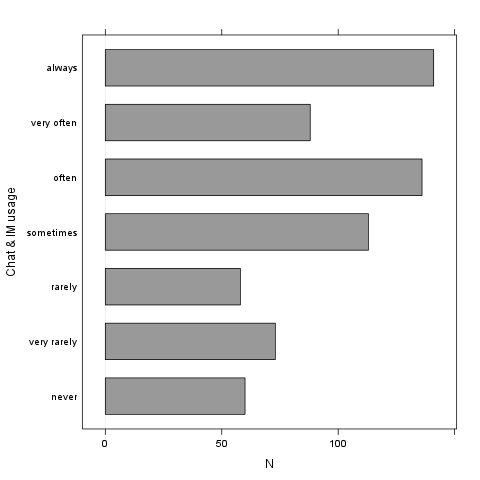
\includegraphics{5a00abbe4c793ceedbbf10939665b5cf.png}
\caption{}
\end{figure}

It seems that the highest value is 7 which is exactly 7 times higher
than the smallest value (1).

\subsubsection{\emph{game} (``On-line games usage'')}

The dataset has 709 observations with 677 valid values (missing: 32) in
\emph{game} (``On-line games usage''). This variable seems to be a
factor.

\paragraph{Base statistics}

\ctable[pos = H, center, botcap]{llllll}
{% notes
}
{% rows
\FL
 & \textbf{game} & \textbf{N} & \textbf{pct} & \textbf{cumul.count} & \textbf{cumul.pct}
\ML
1 & never & 352.00 & 51.99 & 352.00 & 51.99
\\\noalign{\medskip}
2 & very rarely & 128.00 & 18.91 & 480.00 & 70.90
\\\noalign{\medskip}
3 & rarely & 32.00 & 4.73 & 512.00 & 75.63
\\\noalign{\medskip}
4 & sometimes & 60.00 & 8.86 & 572.00 & 84.49
\\\noalign{\medskip}
5 & often & 37.00 & 5.47 & 609.00 & 89.96
\\\noalign{\medskip}
6 & very often & 35.00 & 5.17 & 644.00 & 95.13
\\\noalign{\medskip}
7 & always & 33.00 & 4.87 & 677.00 & 100.00
\\\noalign{\medskip}
Total &  & 677.00 & 100.00 & 677.00 & 100.00
\LL
}

\paragraph{Barplot}

\begin{figure}[htbp]
\centering
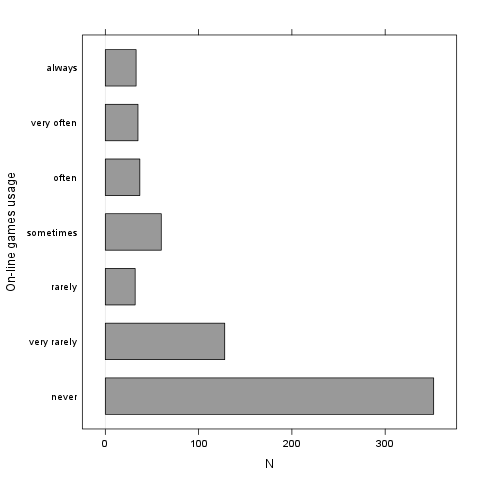
\includegraphics{e53046a09491443064e085131e547971.png}
\caption{}
\end{figure}

It seems that the highest value is 7 which is exactly 7 times higher
than the smallest value (1).

\subsubsection{\emph{surf} (``Web surfing usage'')}

The dataset has 709 observations with 678 valid values (missing: 31) in
\emph{surf} (``Web surfing usage''). This variable seems to be a factor.

\paragraph{Base statistics}

\ctable[pos = H, center, botcap]{llllll}
{% notes
}
{% rows
\FL
 & \textbf{surf} & \textbf{N} & \textbf{pct} & \textbf{cumul.count} & \textbf{cumul.pct}
\ML
1 & never & 17.00 & 2.51 & 17.00 & 2.51
\\\noalign{\medskip}
2 & very rarely & 26.00 & 3.83 & 43.00 & 6.34
\\\noalign{\medskip}
3 & rarely & 33.00 & 4.87 & 76.00 & 11.21
\\\noalign{\medskip}
4 & sometimes & 107.00 & 15.78 & 183.00 & 26.99
\\\noalign{\medskip}
5 & often & 158.00 & 23.30 & 341.00 & 50.29
\\\noalign{\medskip}
6 & very often & 142.00 & 20.94 & 483.00 & 71.24
\\\noalign{\medskip}
7 & always & 195.00 & 28.76 & 678.00 & 100.00
\\\noalign{\medskip}
Total &  & 678.00 & 100.00 & 678.00 & 100.00
\LL
}

\paragraph{Barplot}

\begin{figure}[htbp]
\centering
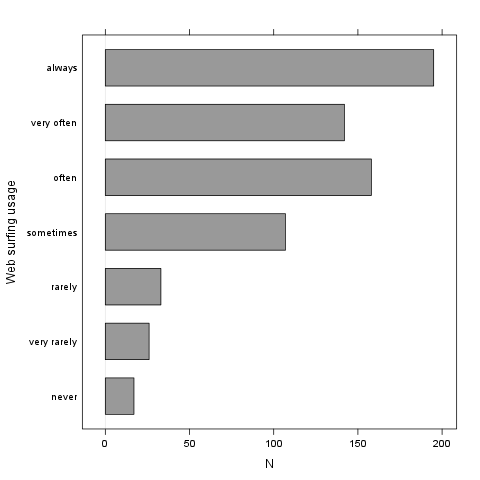
\includegraphics{0166a8b5df2f3db871e8736bfee8af6e.png}
\caption{}
\end{figure}

It seems that the highest value is 7 which is exactly 7 times higher
than the smallest value (1).

\subsubsection{\emph{email} (``Email usage'')}

The dataset has 709 observations with 672 valid values (missing: 37) in
\emph{email} (``Email usage''). This variable seems to be a factor.

\paragraph{Base statistics}

\ctable[pos = H, center, botcap]{llllll}
{% notes
}
{% rows
\FL
 & \textbf{email} & \textbf{N} & \textbf{pct} & \textbf{cumul.count} & \textbf{cumul.pct}
\ML
1 & never & 13.00 & 1.93 & 13.00 & 1.93
\\\noalign{\medskip}
2 & very rarely & 36.00 & 5.36 & 49.00 & 7.29
\\\noalign{\medskip}
3 & rarely & 46.00 & 6.85 & 95.00 & 14.14
\\\noalign{\medskip}
4 & sometimes & 87.00 & 12.95 & 182.00 & 27.08
\\\noalign{\medskip}
5 & often & 123.00 & 18.30 & 305.00 & 45.39
\\\noalign{\medskip}
6 & very often & 108.00 & 16.07 & 413.00 & 61.46
\\\noalign{\medskip}
7 & always & 259.00 & 38.54 & 672.00 & 100.00
\\\noalign{\medskip}
Total &  & 672.00 & 100.00 & 672.00 & 100.00
\LL
}

\paragraph{Barplot}

\begin{figure}[htbp]
\centering
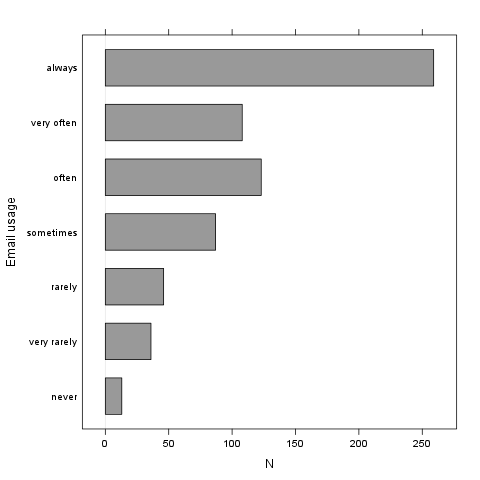
\includegraphics{895cde198b269bf65b01e1e067a515c8.png}
\caption{}
\end{figure}

It seems that the highest value is 7 which is exactly 7 times higher
than the smallest value (1).

\subsubsection{\emph{download} (``Download usage'')}

The dataset has 709 observations with 677 valid values (missing: 32) in
\emph{download} (``Download usage''). This variable seems to be a
factor.

\paragraph{Base statistics}

\ctable[pos = H, center, botcap]{llllll}
{% notes
}
{% rows
\FL
 & \textbf{download} & \textbf{N} & \textbf{pct} & \textbf{cumul.count} & \textbf{cumul.pct}
\ML
1 & never & 11.00 & 1.62 & 11.00 & 1.62
\\\noalign{\medskip}
2 & very rarely & 28.00 & 4.14 & 39.00 & 5.76
\\\noalign{\medskip}
3 & rarely & 29.00 & 4.28 & 68.00 & 10.04
\\\noalign{\medskip}
4 & sometimes & 80.00 & 11.82 & 148.00 & 21.86
\\\noalign{\medskip}
5 & often & 124.00 & 18.32 & 272.00 & 40.18
\\\noalign{\medskip}
6 & very often & 160.00 & 23.63 & 432.00 & 63.81
\\\noalign{\medskip}
7 & always & 245.00 & 36.19 & 677.00 & 100.00
\\\noalign{\medskip}
Total &  & 677.00 & 100.00 & 677.00 & 100.00
\LL
}

\paragraph{Barplot}

\begin{figure}[htbp]
\centering
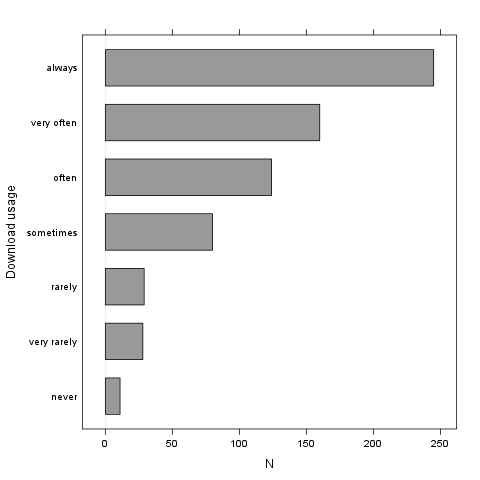
\includegraphics{dde181184885b8777d0248b3f421289a.png}
\caption{}
\end{figure}

It seems that the highest value is 7 which is exactly 7 times higher
than the smallest value (1).

\subsubsection{\emph{forum} (``Web forums usage'')}

The dataset has 709 observations with 673 valid values (missing: 36) in
\emph{forum} (``Web forums usage''). This variable seems to be a factor.

\paragraph{Base statistics}

\ctable[pos = H, center, botcap]{llllll}
{% notes
}
{% rows
\FL
 & \textbf{forum} & \textbf{N} & \textbf{pct} & \textbf{cumul.count} & \textbf{cumul.pct}
\ML
1 & never & 76.00 & 11.29 & 76.00 & 11.29
\\\noalign{\medskip}
2 & very rarely & 80.00 & 11.89 & 156.00 & 23.18
\\\noalign{\medskip}
3 & rarely & 72.00 & 10.70 & 228.00 & 33.88
\\\noalign{\medskip}
4 & sometimes & 111.00 & 16.49 & 339.00 & 50.37
\\\noalign{\medskip}
5 & often & 109.00 & 16.20 & 448.00 & 66.57
\\\noalign{\medskip}
6 & very often & 119.00 & 17.68 & 567.00 & 84.25
\\\noalign{\medskip}
7 & always & 106.00 & 15.75 & 673.00 & 100.00
\\\noalign{\medskip}
Total &  & 673.00 & 100.00 & 673.00 & 100.00
\LL
}

\paragraph{Barplot}

\begin{figure}[htbp]
\centering
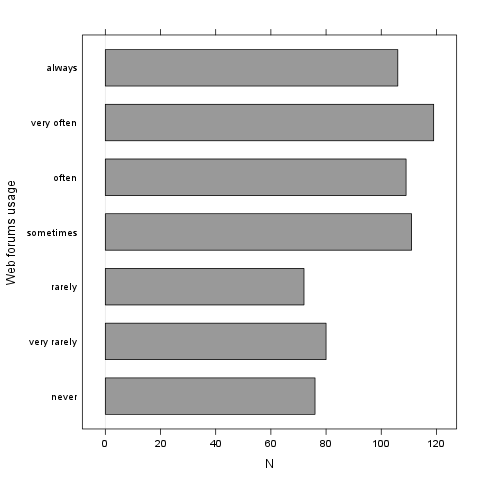
\includegraphics{ac419134b2f4695e544d8886ba12e0c2.png}
\caption{}
\end{figure}

It seems that the highest value is 7 which is exactly 7 times higher
than the smallest value (1).

\subsubsection{\emph{socnet} (``Social networks usage'')}

The dataset has 709 observations with 678 valid values (missing: 31) in
\emph{socnet} (``Social networks usage''). This variable seems to be a
factor.

\paragraph{Base statistics}

\ctable[pos = H, center, botcap]{llllll}
{% notes
}
{% rows
\FL
 & \textbf{socnet} & \textbf{N} & \textbf{pct} & \textbf{cumul.count} & \textbf{cumul.pct}
\ML
1 & never & 208.00 & 30.68 & 208.00 & 30.68
\\\noalign{\medskip}
2 & very rarely & 102.00 & 15.04 & 310.00 & 45.72
\\\noalign{\medskip}
3 & rarely & 57.00 & 8.41 & 367.00 & 54.13
\\\noalign{\medskip}
4 & sometimes & 87.00 & 12.83 & 454.00 & 66.96
\\\noalign{\medskip}
5 & often & 79.00 & 11.65 & 533.00 & 78.61
\\\noalign{\medskip}
6 & very often & 80.00 & 11.80 & 613.00 & 90.41
\\\noalign{\medskip}
7 & always & 65.00 & 9.59 & 678.00 & 100.00
\\\noalign{\medskip}
Total &  & 678.00 & 100.00 & 678.00 & 100.00
\LL
}

\paragraph{Barplot}

\begin{figure}[htbp]
\centering
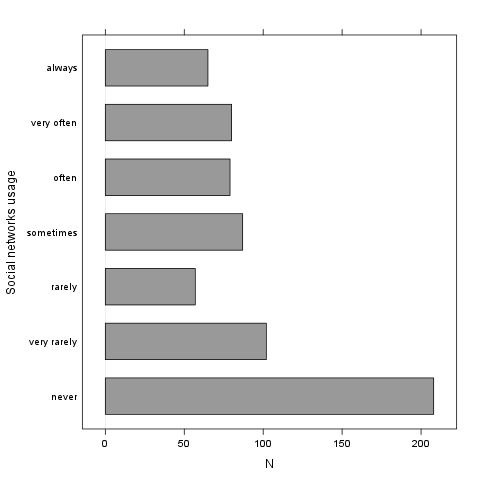
\includegraphics{8475d98870c1cdd2436a3abdb0d69a66.png}
\caption{}
\end{figure}

It seems that the highest value is 7 which is exactly 7 times higher
than the smallest value (1).

\subsubsection{\emph{xxx} (``Adult sites usage'')}

The dataset has 709 observations with 674 valid values (missing: 35) in
\emph{xxx} (``Adult sites usage''). This variable seems to be a factor.

\paragraph{Base statistics}

\ctable[pos = H, center, botcap]{llllll}
{% notes
}
{% rows
\FL
 & \textbf{xxx} & \textbf{N} & \textbf{pct} & \textbf{cumul.count} & \textbf{cumul.pct}
\ML
1 & never & 274.00 & 40.65 & 274.00 & 40.65
\\\noalign{\medskip}
2 & very rarely & 124.00 & 18.40 & 398.00 & 59.05
\\\noalign{\medskip}
3 & rarely & 52.00 & 7.72 & 450.00 & 66.77
\\\noalign{\medskip}
4 & sometimes & 131.00 & 19.44 & 581.00 & 86.20
\\\noalign{\medskip}
5 & often & 46.00 & 6.82 & 627.00 & 93.03
\\\noalign{\medskip}
6 & very often & 28.00 & 4.15 & 655.00 & 97.18
\\\noalign{\medskip}
7 & always & 19.00 & 2.82 & 674.00 & 100.00
\\\noalign{\medskip}
Total &  & 674.00 & 100.00 & 674.00 & 100.00
\LL
}

\paragraph{Barplot}

\begin{figure}[htbp]
\centering
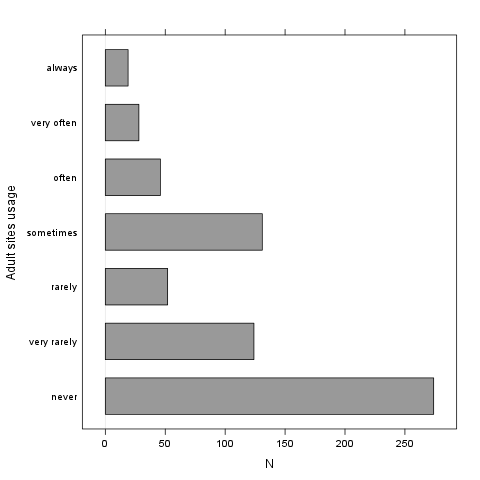
\includegraphics{4fda8cf992e8de93624c45ef3c72a0c5.png}
\caption{}
\end{figure}

It seems that the highest value is 7 which is exactly 7 times higher
than the smallest value (1).

\end{document}
